%!TEX root=rapport.tex

\section{Interprétation des résultats obtenus}

\subsection{Résultats finaux}

Pour étudier les résultats que notre programme nous retourne, nous avons utilisé
un \textit{dotmatcher}.
Le principe du dotmatcher est de comparer deux séquences $s$ et $t$ données en
entrée: le dotmatcher parcourt les séquences en comparant chaque nucléotide
entre eux.  Lorsqu'une correspondance est faite, un point est tracé sur un
graphique. Une option, appelée \textit{thresold} peut être ajustée pour dissiper
le bruit. Une valeur de 50 a été utilisée pour l'option \textit{threshold}.

Pour chaque nucléotide $s_{i}$ de la séquence $s$ et chaque nucléotide $t_{j}$
de la séquence $t$, le dotmatcher va tracer un point s'il y a une correspondance
entre les deux nucléotides.

Pour chaque comparaison de séquences, nous obtenons donc un rectangle de
points. Sur l'axe X, nous avons la longueur de la séquence que nous devons
obtenir, et sur l'axe Y, nous avons la longueur de la séquence que nous avons
obtenue.

Nous souhaitons, à travers ces graphiques, étudier la qualité de notre
résultat en regardant si chaque morceau de la séquence cible est bien
atteinte. Ceci se remarque par la présence de segments de droites car ceux-ci
reflètent une suite de nucléotides qui correspondent. Pour cela, il
suffit de projeter chaque segment obtenu sur l'axe X et regarder si l'ensemble
recouvre globalement la séquence de départ.

\subsubsection*{Cible 1}

Au niveau de la première cible (voir figure~\ref{cible1}), nous remarquons d'abord que la séquence que nous
avons obtenue est plus longue que la séquence cible fournie ($\simeq$ 14 000 vs
$\simeq$ 9000).

Les résultats sont meilleurs pour le normal que pour son complémentaire
inversé. Le recouvrement du premier est presque global, les intervalles non
couverts se trouvant aux alentours de 1000 et 7000. Quant au complémentaire
inversé, il y a un intervalle non couvert entre 2000 et 4000 ainsi que des
petits intervalles entre chaque segment.

Nous remarquons, à travers les droites, que nous avons de longues successions de
correspondances.

\begin{figure}[!ht]
	\begin{minipage}[r]{.46\linewidth}
		\begin{center}
		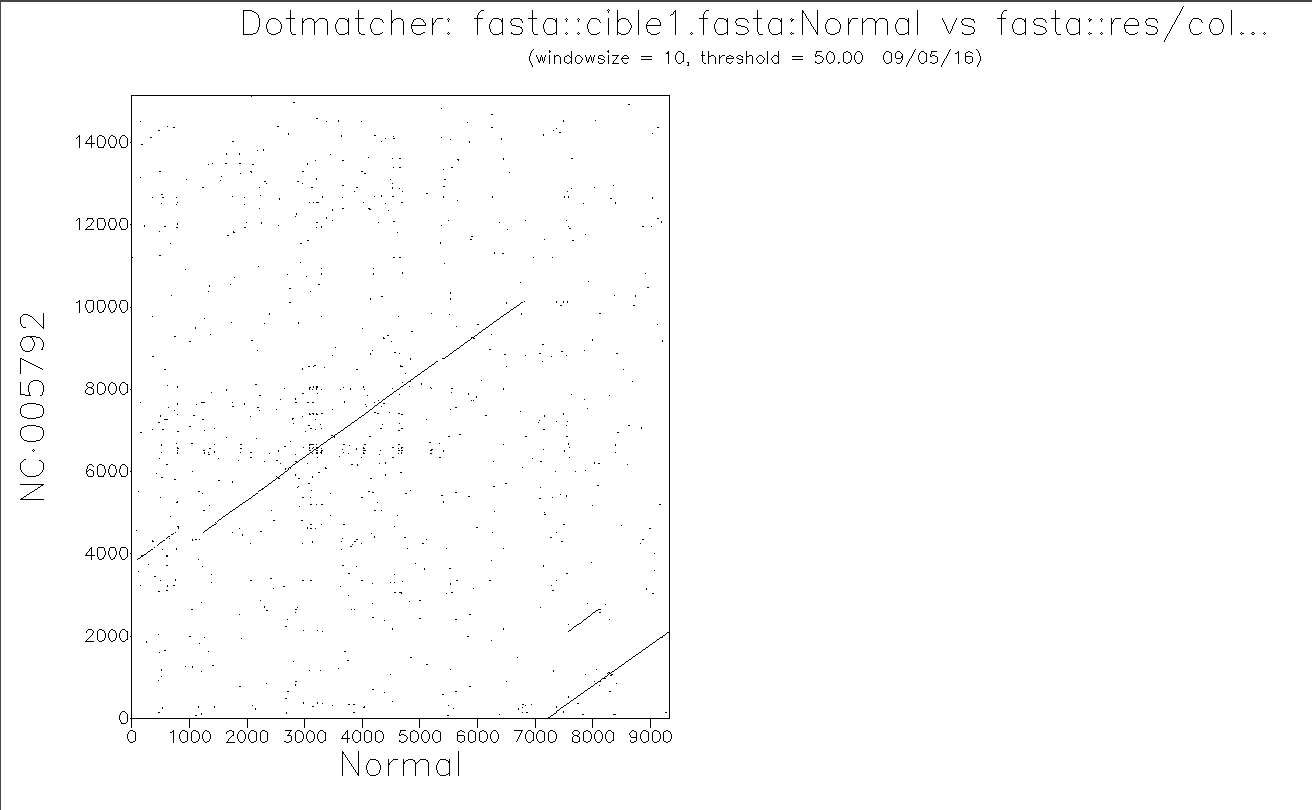
\includegraphics[scale= 0.7]{../res/cible1.png}
		Sequence obtenue
			\end{center}
\end{minipage} \hfill
\begin{minipage}[c]{.46 \linewidth}
	\begin{center}
			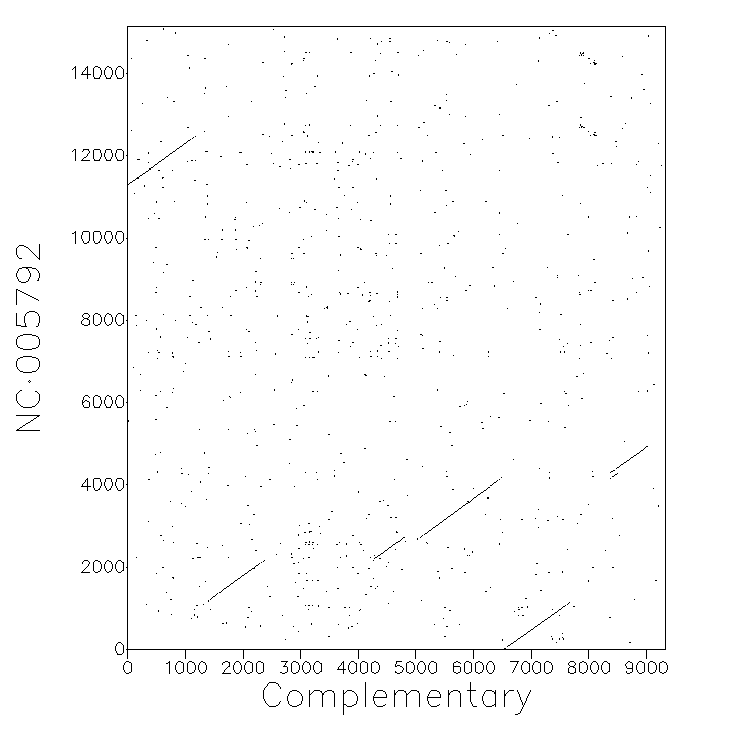
\includegraphics[scale= 0.7]{../res/cible1-ic.png}
			 Séquence complémentée et inversée
		\end{center}
	\end{minipage}
	\caption{Résultat de la collection 1}
	\label{cible1}
\end{figure}

\FloatBarrier

\subsubsection*{Cible 2}

Quant à la seconde cible (voir figure~\ref{cible2}), nous pouvons remarquer qu'il y a peu de
correspondances. Cependant, si nous zoomons sur certaines zones, nous pouvons
voir apparaitre des petits segments de droites.

Nous obtenons également une plus grande séquence: la cible contient environ
118000 nucléotides tandis que notre alignement en contient 190000.

\begin{figure}[!ht]
	\begin{minipage}[r]{.46\linewidth}
		\begin{center}
		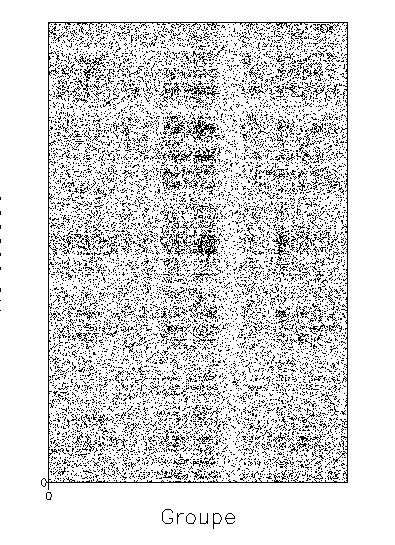
\includegraphics[scale=0.7]{../res/cible2.png}
Séquence obtenue	\end{center}
\end{minipage} \hfill
\begin{minipage}[c]{.46 \linewidth}
	\begin{center}
			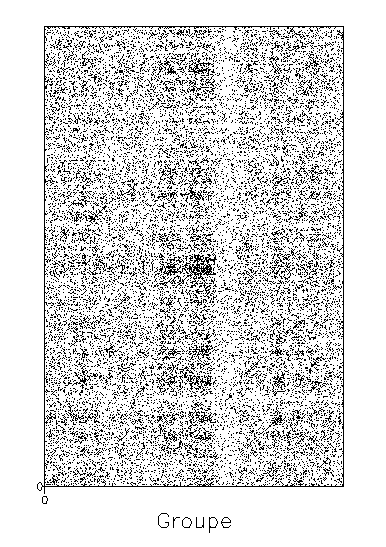
\includegraphics[scale=0.7]{../res/cible2-ic.png}
			 Séquence complémentée et inversée
		\end{center}
	\end{minipage}
	\caption{Résultat de la collection 2}
	\label{cible2}
\end{figure}

\FloatBarrier

\subsubsection*{Cible 4}

Les résultats pour la cible 4 (voir figure~\ref{cible4}) sont plutôt satisfaisants comme pour les cibles 1
et 5. Nous obtenons un recouvrement quasi-global ainsi qu'une longue droite
recouvrant environ 65\% de la séquence cible.

Pour son complémentaire inversé, le recouvrement est plus éparpillé mais reste
tout de même assez global.

Comme les 2 premières séquences, nous obtenons une séquence plus longue.

\begin{figure}[!ht]
	\begin{minipage}[r]{.46\linewidth}
		\begin{center}
		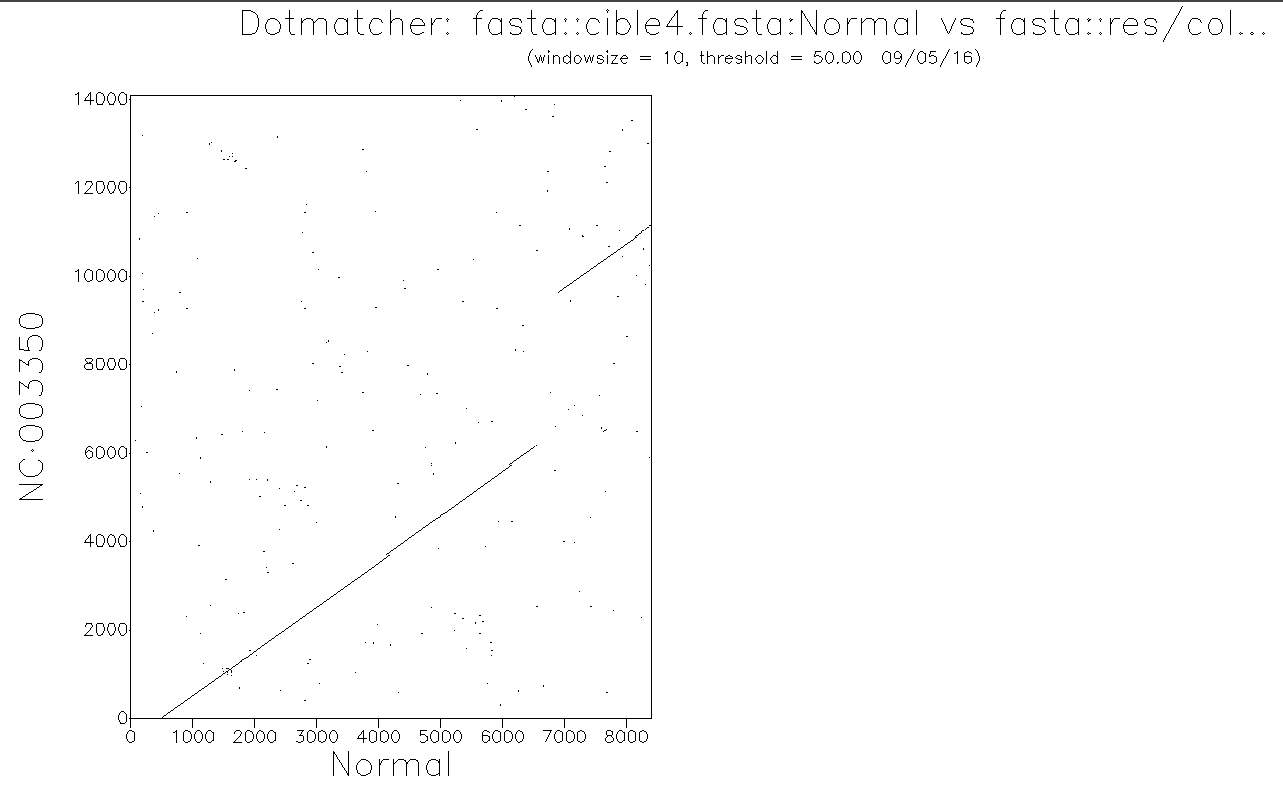
\includegraphics[scale= 0.7]{../res/cible4.png}
Séquence obtenue	\end{center}
\end{minipage} \hfill
\begin{minipage}[c]{.46 \linewidth}
	\begin{center}
			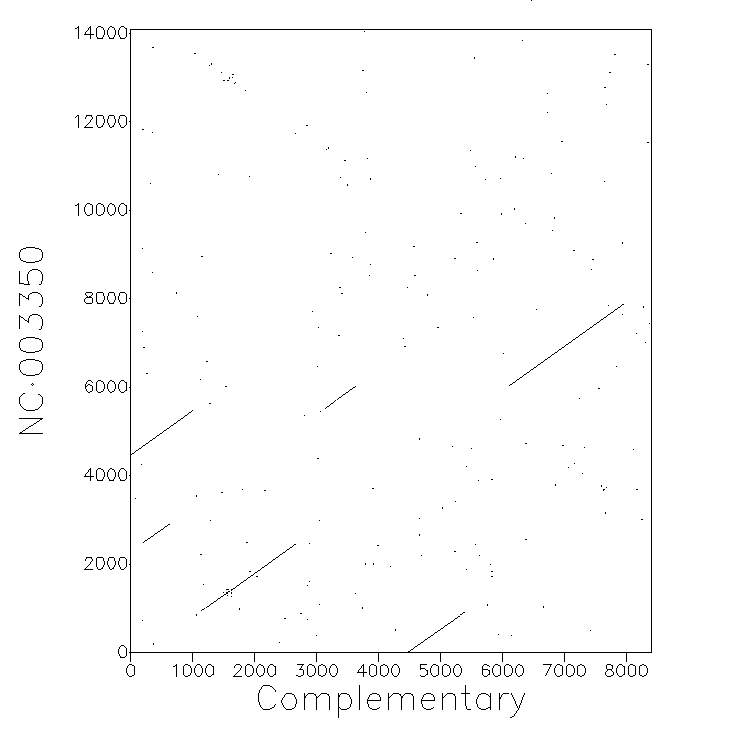
\includegraphics[scale= 0.7]{../res/cible4-ic.png}
			 Séquence complémentée et inversée
		\end{center}
	\end{minipage}
	\caption{Résultat de la collection 4}
	\label{cible4}
\end{figure}

\FloatBarrier

\subsubsection*{Cible 5}


Pour la dernière cible (voir figure~\ref{cible5}), nous obtenons aussi plusieurs segments de droites,
plus ou moins grands, recouvrant la majorité de la séquence cible (un peu plus
de 90\%). Les endroits où les deux séquences ne correspondent pas se situent aux
alentours de 3000 et 7500. Le complémentaire inversé remplit également une bonne
partie de la séquence cible mais il y a plus d'intervalles où les séquences ne
correspondent pas.

Comme pour les séquences précédentes, notre algorithme nous renvoie une séquence
plus longue (environ 6000 nucléotides de plus).

\begin{figure}[!ht]
	\begin{minipage}[r]{.46\linewidth}
		\begin{center}
		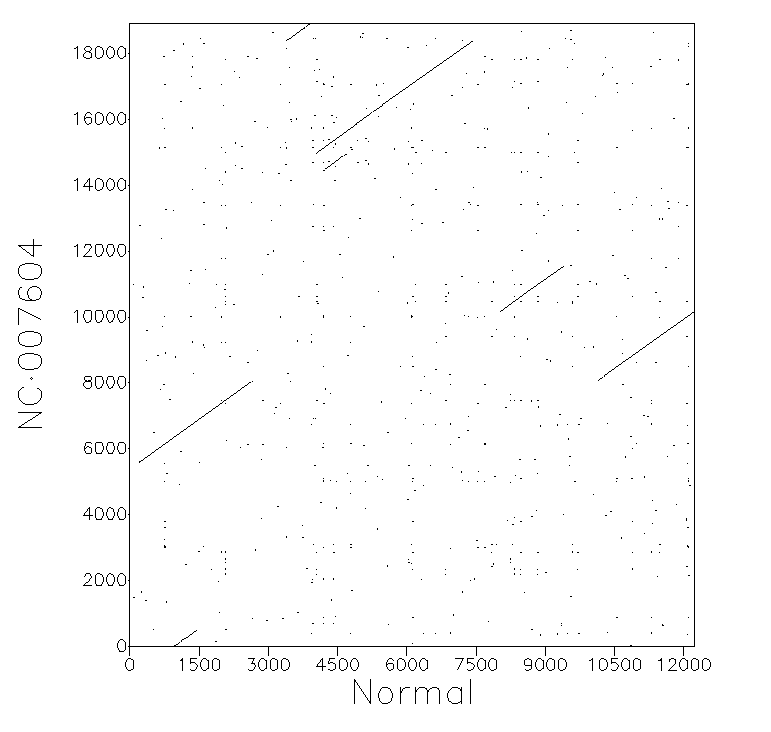
\includegraphics[scale= 0.7]{../res/cible5.png}
Séquence obtenue	\end{center}
\end{minipage} \hfill
\begin{minipage}[c]{.46 \linewidth}
	\begin{center}
			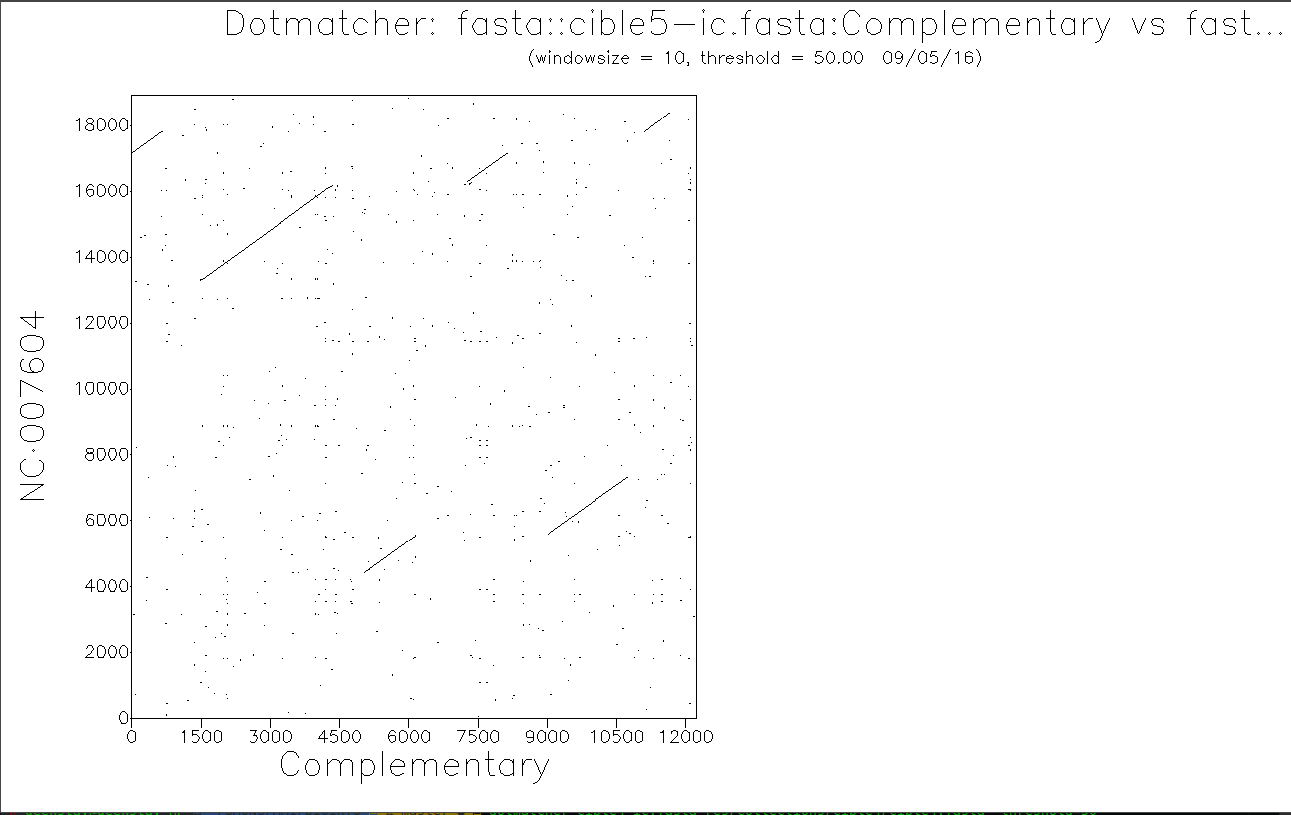
\includegraphics[scale= 0.7]{../res/cible5-ic.png}
			 Séquence complémentée et inversée
		\end{center}
	\end{minipage}
	\caption{Résultat de la collection 5}
	\label{cible5}
\end{figure}

\FloatBarrier


\subsubsection*{Interprétation générale}

De manière générale, nous recouvrons globalement chaque séquence, (jusqu'à 90\%
pour la cible 4), soit de manière continue (longue droite, comme les cibles 1 et
4), soit un peu éparpillé (segments de droite recouvrant de 10 à 40\%, cible 5),
soit très peu de segments et très éparpillé (très petits segments de droites lors
du zoom, cible 2).

Chaque séquence obtenue est plus grande que la séquence cible.

\subsection{Autres implémentations}

Nous avons également expérimenté le changement de \og comportement \fg~de l'algorithme glouton en modifiant
le comparateur d'arcs pour privilégier les alignements ayant une plus grande
sous-séquence commune.

Lorsque deux arcs ont un même score d'alignement, nous avons pour cela
privilégié les arcs qui ont une plus longue sous-séquence commune. Cette méthode
nous a donné des résultats équivalents si ce n'est que les droites apparaissent
plus bas sur le graphe. Sur la figure \ref{fig:autre_impl_4} est représentée le
dotmatcher obtenu sur la collection 4 avec ce nouveau comparateur d'arc. Les
autres dotmatchers donnent la même chose si ce n'est que la projection des segments sur l'axe Y n'est pas au même endroit.

\begin{figure}[!ht]
	\begin{minipage}[r]{.46\linewidth}
		\begin{center}
			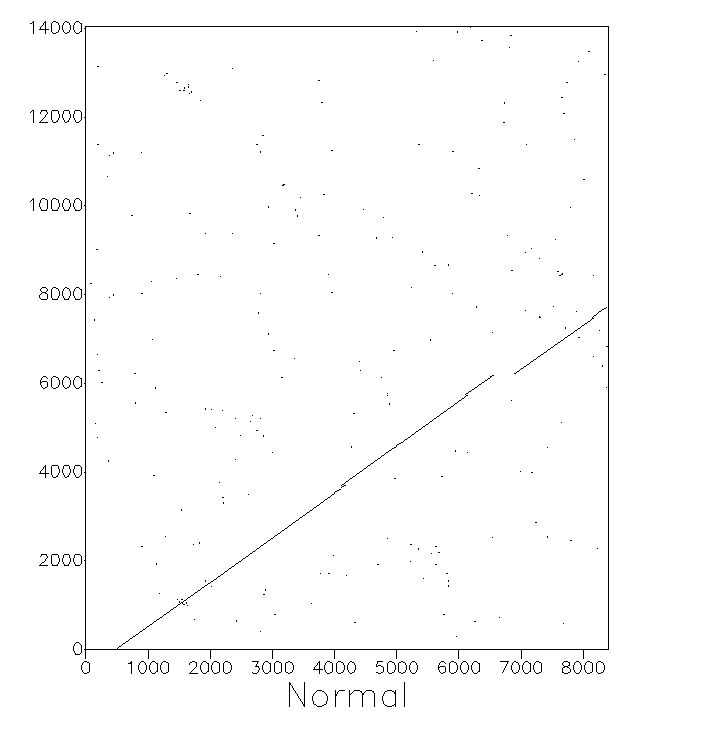
\includegraphics[scale= 0.4]{../res/cible4-other.png}
			Autre implémentation: collection 4
		\end{center}
	\end{minipage} \hfill
	\begin{minipage}[c]{.46\linewidth}
		\begin{center}
		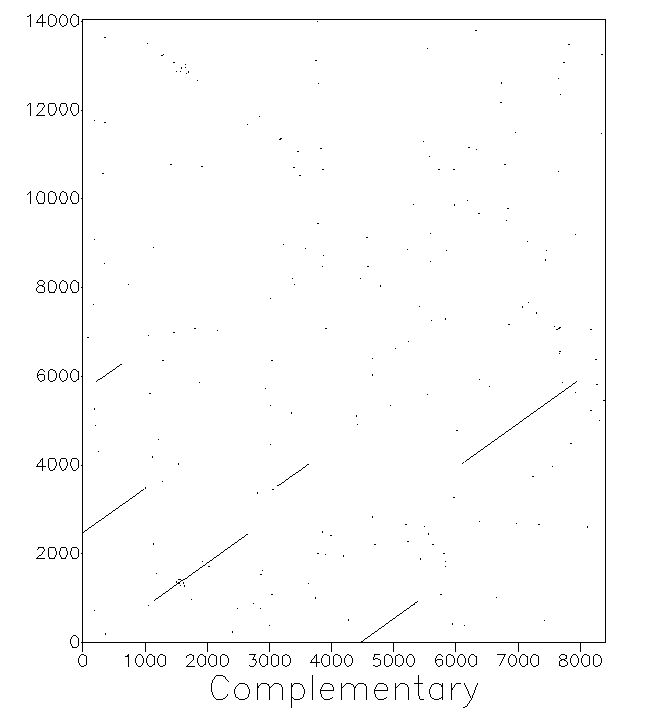
\includegraphics[scale= 0.4]{../res/cible4-ic-other.png}
		Autre implémentation: collection 4, complémenté et inversé
	\end{center}
	\end{minipage}
	\label{fig:autre_impl_4}
	\caption{Autre implémentation: collection 4}
\end{figure}

\FloatBarrier

Dans le code soumis, nous avons prévilégié, lors de l'alignement semi-global,
l'alignement avec le moins de gaps finaux et initiaux, c'est-à-dire en
prenant le dernier maximum pour la dernière colonne et la dernière ligne. Nous
avons tenté de prendre le premier maximum pour chacun d'entre eux, mais cela n'a
pas donné de meilleurs résultats.

%Explication de la propagations des gaps à la fin.
